% Solution: Tadelis (2013) Exercise 7.2 "Strategies and Equilibrium". Input by \solitem.
% New in the 30-item list. Check: check_B_L03.py.
\begin{exsol}{Tadelis Exercise 7.2}{147}{Foundations}{2}
\asked For the three-move game $A/B$, then $C/D$, then $E/F$: (a) its tree and type of
information; (b) terminal nodes and information sets; (c) pure strategies per player; (d) with
the given payoffs, all Nash equilibria and which one is more appealing.

\method Game tree and information sets (Lecture~3, slides~20--23; Tadelis \S7.1, Defs.~7.1--7.2,
pp.~133--135); perfect information (slide~24; Def.~7.3, p.~136); pure strategies as complete plans
(slide~25; Def.~7.4, p.~138); the normal form of an extensive-form game (Tadelis \S7.2.3,
pp.~142--145); Nash equilibria by best-reply marking and indifference; the ``appealing'' one by
sequential rationality and backward induction (slides~29--30; Tadelis \S8.1, pp.~152--153).

\solution
\textbf{(a) Tree.} Payoffs $(u_1,u_2)$ from part (d) are written at the leaves.
\begin{center}
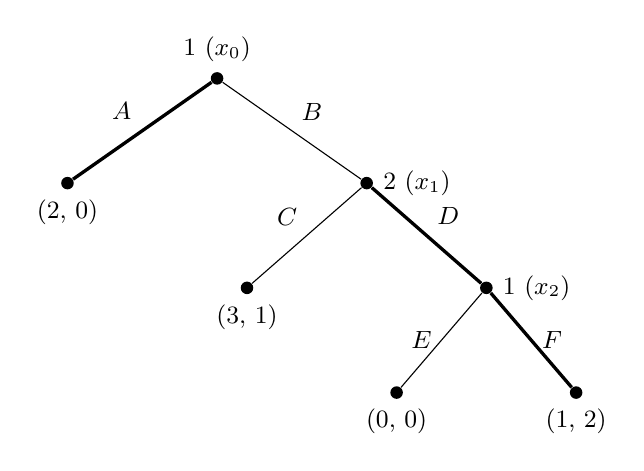
\begin{tikzpicture}[scale=0.95,dot/.style={circle,fill,inner sep=1.6pt},
  every node/.style={font=\small}]
  \node[dot,label=above:{1 ($x_0$)}] (r) at (0,0) {};
  \node[dot,label=below:{$(2,\,0)$}] (a) at (-2,-1.4) {};
  \node[dot,label=right:{2 ($x_1$)}] (x1) at (2,-1.4) {};
  \node[dot,label=below:{$(3,\,1)$}] (c) at (0.4,-2.8) {};
  \node[dot,label=right:{1 ($x_2$)}] (x2) at (3.6,-2.8) {};
  \node[dot,label=below:{$(0,\,0)$}] (e) at (2.4,-4.2) {};
  \node[dot,label=below:{$(1,\,2)$}] (f) at (4.8,-4.2) {};
  \draw[very thick] (r) -- node[above left] {$A$} (a);
  \draw (r) -- node[above right] {$B$} (x1);
  \draw (x1) -- node[above left] {$C$} (c);
  \draw[very thick] (x1) -- node[above right] {$D$} (x2);
  \draw (x2) -- node[left] {$E$} (e);
  \draw[very thick] (x2) -- node[right] {$F$} (f);
\end{tikzpicture}\\[2pt]
{\footnotesize Thick branches = backward-induction choices (part (d)).}
\end{center}
Each decision node is alone in its information set (the mover always knows the history), so it is
a game of \textbf{perfect information}.

\textbf{(b) Counts.} Terminal nodes: the leaves after $A$, $C$, $E$, $F$, so \textbf{4}.
Information sets: $\{x_0\}$, $\{x_2\}$ for player~1 and $\{x_1\}$ for player~2, so \textbf{3}
(two for player~1, one for player~2).

\textbf{(c) Pure strategies.} Player~1 picks an action at $x_0$ and at $x_2$, even when his
first action ($A$) makes $x_2$ unreachable: $S_1 = \{AE, AF, BE, BF\}$, \textbf{4} strategies
($2 \times 2$, item ``Tadelis 7.1''). Player~2 has one information set: $S_2 = \{C, D\}$,
\textbf{2} strategies.

\textbf{(d) Nash equilibria.} Normal form (rows player~1, columns player~2):
\begin{center}
\begin{tabular}{r|c|c|}
\multicolumn{1}{r}{} & \multicolumn{1}{c}{$C$} & \multicolumn{1}{c}{$D$}\\ \cline{2-3}
$AE$ & $2,\ \br{0}$ & $\br{2},\ \br{0}$ \\ \cline{2-3}
$AF$ & $2,\ \br{0}$ & $\br{2},\ \br{0}$ \\ \cline{2-3}
$BE$ & $\br{3},\ \br{1}$ & $0,\ 0$ \\ \cline{2-3}
$BF$ & $\br{3},\ 1$ & $1,\ \br{2}$ \\ \cline{2-3}
\end{tabular}
\end{center}
\emph{Pure Nash equilibria} (both payoffs underlined): $(AE, D)$, $(AF, D)$ and $(BE, C)$.
$(BF, C)$ fails because against $BF$ player~2 prefers $D$ ($2 > 1$).

\emph{All Nash equilibria.} Let $q = \Pr_2(C)$. Player~1's payoffs are
\[
  u_1(AE) = u_1(AF) = 2, \qquad u_1(BE) = 3q, \qquad u_1(BF) = 3q + (1-q) = 1 + 2q .
\]
\begin{itemize}
  \item $q < \frac12$: $2 > 1 + 2q > 3q$, so player~1 plays $A$ (any mix of $AE$, $AF$); player~2's
  node is not reached, she is indifferent, and any such $q$ is a best reply. \emph{Equilibria.}
  \item $q = \frac12$: $AE$, $AF$, $BF$ tie at 2. If $BF$ had positive weight, player~2's node would
  be reached only after $BF$, where $D$ is strictly better ($2 > 1$), forcing $q = 0$. So player~1
  stays on $\{AE, AF\}$. \emph{Equilibria.}
  \item $\frac12 < q < 1$: $1 + 2q > \max\{2, 3q\}$, so $BF$ is the unique best reply, and then
  $q = 0$. Contradiction.
  \item $q = 1$: $BE$ and $BF$ tie at 3 > 2. With $w = \Pr_1(BF)$ (the rest on $BE$), player~2
  gets $1$ from $C$ and $2w$ from $D$, so $C$ is a best reply iff $w \le \frac12$. \emph{Equilibria.}
\end{itemize}
Hence the set of Nash equilibria is
\[
  \bigl\{(\text{any mix of } AE, AF;\ q) : 0 \le q \le \tfrac12\bigr\}
  \;\cup\; \bigl\{((1-w)\,BE + w\,BF;\ C) : 0 \le w \le \tfrac12\bigr\},
\]
with outcome $A$ and payoffs $(2,0)$ in the first family and outcome $(B, C)$, payoffs $(3,1)$, in
the second.

\emph{The appealing one.} Backward induction: at $x_2$ player~1 picks $F$ ($1 > 0$); at $x_1$
player~2, anticipating $F$, compares $C \mapsto 1$ with $D \mapsto 2$ and picks $D$; at $x_0$
player~1 compares $A \mapsto 2$ with $B \mapsto 1$ and picks $A$. The backward-induction profile,
and the unique SPE, is $(AF, D)$, outcome $A$, payoffs $(2, 0)$. It is the appealing one because
every player's plan is optimal at every node, reached or not. The other two pure equilibria rely
on player~1's plan to play $E$ at $x_2$, which gives him $0 < 1$:
\begin{itemize}
  \item in $(BE, C)$ the plan $E$ is a \emph{threat} that scares player~2 into $C$; if $x_2$ were
  reached, player~1 would not carry it out;
  \item in $(AE, D)$ the plan $E$ is never tested and does not change the outcome, but it is still
  not sequentially rational.
\end{itemize}

\interp Player~1 would like to commit to $E$ (``if you play $D$ I will burn both our payoffs''),
because that threat earns him 3 instead of 2. He cannot: at $x_2$ the damage is in the past and
$F$ is better. Nash equilibrium accepts the threat because $x_2$ is off the path; sequential
rationality rejects it. This is the Brexit pattern of Lecture~4 (slides~8--13): several Nash
equilibria are held up by threats nobody would execute, and only the backward-induction profile
survives.

\verify \texttt{check\_B\_L03.py} runs backward induction on the tree (unique solution, outcome
$A$, payoffs $(2,0)$; continuation $D$ then $F$ after $B$), finds the three pure Nash equilibria of
the $4\times2$ matrix, scans $q$ on a grid of step $\frac1{120}$ plus $\frac12, \frac23$ (Nash
equilibria exist exactly for $q \le \frac12$ and $q = 1$), and tests the $w \le \frac12$
condition on a grid. Output line: \texttt{tadelis-7-2: SPE (AF, D); pure NE (AE,D), (AF,D),
(BE,C)}. Tadelis prints no answer.

\mistakes
\begin{itemize}
  \item Giving player~1 only three strategies ($A$, $BE$, $BF$). That is the reduced normal form;
  as Tadelis defines strategies, $A$ must be completed with a plan at $x_2$.
  \item Calling $(BE, C)$ the ``best'' equilibrium because it gives player~1 more. A Nash
  equilibrium is appealing when its threats are credible, not when it pays one player more.
  \item Counting 3 information sets as ``3 decision nodes per player'' or counting terminal nodes
  as information sets.
\end{itemize}

\answer{(a) Tree above; perfect information. (b) 4 terminal nodes; 3 information sets (2 for
player~1, 1 for player~2). (c) Player~1: 4 ($AE, AF, BE, BF$); player~2: 2 ($C, D$). (d) Pure
Nash equilibria $(AE, D)$, $(AF, D)$, $(BE, C)$ (plus mixed ones: player~1 on $A$ with
$\Pr(C) \le \frac12$, or $(1-w)BE + wBF$ with $w \le \frac12$ against $C$). The appealing one is
$(AF, D)$, the unique SPE: the others rest on the non-credible plan $E$.}
\end{exsol}
